\documentclass[11pt,twoside,a4paper]{article}
% http://www-h.eng.cam.ac.uk/help/tpl/textprocessing/latex_maths+pix/node6.html symboles de math
% http://fr.wikibooks.org/wiki/Programmation_LaTeX Programmation latex (wikibook)
%=========================== En-Tete =================================
%--- Insertion de paquetages (optionnel) ---
\usepackage[french]{babel}   % pour dire que le texte est en fran{\'e}ais
\usepackage{a4}	             % pour la taille   
\usepackage[T1]{fontenc}     % pour les font postscript
\usepackage{epsfig}          % pour gerer les images
%\usepackage{psfig}
\usepackage{amsmath, amsthm} % tres bon mode mathematique
\usepackage{amsfonts,amssymb}% permet la definition des ensembles
\usepackage{float}           % pour le placement des figure
\usepackage{verbatim}

\usepackage{longtable}		% pour les tableaux de plusieurs pages

\usepackage[table]{xcolor}	% couleur de fond des cellules de tableaux

\usepackage{lastpage}

\usepackage{multirow}

\usepackage{multicol} % pour {\'e}crire dans certaines zones en colonnes : \begin{multicols}{nb colonnes}...\end{multicols} 

% \usepackage[top=1.5cm, bottom=1.5cm, left=1.5cm, right=1.5cm]{geometry}
% gauche, haut, droite, bas, entete, ente2txt, pied, txt2pied
\usepackage{vmargin}
\setmarginsrb{0.20cm}{0.20cm}{0.20cm}{0.20cm}{15pt}{3pt}{15pt}{3pt}

\usepackage{lscape} % changement orientation page
%\usepackage{frbib} % enlever pour obtenir references en anglais
% --- style de page (pour les en-tete) ---
\pagestyle{empty}

% % % en-tete et pieds de page configurables : fancyhdr.sty

% http://www.trustonme.net/didactels/250.html

% http://ww3.ac-poitiers.fr/math/tex/pratique/entete/entete.htm
% http://www.ctan.org/tex-archive/macros/latex/contrib/fancyhdr/fancyhdr.pdf
% \usepackage{fancyhdr}
% \pagestyle{fancy}
% % \newcommand{\chaptermark}[1]{\markboth{#1}{}}
% % \newcommand{\sectionmark}[1]{\markright{\thesection\ #1}}
% \fancyhf{}
% \fancyhead[LE,RO]{\bfseries\thepage}
% \fancyhead[LO]{\bfseries\rightmark}
% \fancyhead[RE]{\bfseries\leftmark}
% \fancyfoot[LE]{\thepage /\pageref{LastPage} \hfill
	% TITLE
% \hfill 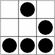
\includegraphics[width=0.5cm]{img/logo_glider.png} }
% \fancyfoot[RO]{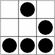
\includegraphics[width=0.5cm]{img/logo_glider.png} \hfill
	% TITLE
% \hfill \thepage /\pageref{LastPage}}
% \renewcommand{\headrulewidth}{0.5pt}
% \renewcommand{\footrulewidth}{0.5pt}
% \addtolength{\headheight}{0.5pt}
% \fancypagestyle{plain}{
	% \fancyhead{}
	% \renewcommand{\headrulewidth}{0pt}
% }

\def\imgPUISSlight{\begin{tabular}[h]{p{0.45cm}} \\ \includegraphics[width=0.50cm]{../../../../../../imgGraphics/rolePlayingGame/SimulacreS/normal40x40/puissanceLIGHT.png}	\\ \end{tabular}}
\def\imgRAPIDlight{\begin{tabular}[h]{p{0.45cm}} \\ \includegraphics[width=0.50cm]{../../../../../../imgGraphics/rolePlayingGame/SimulacreS/normal40x40/rapiditeLIGHT.png}	\\ \end{tabular}}
\def\imgPRECIlight{\begin{tabular}[h]{p{0.45cm}} \\ \includegraphics[width=0.50cm]{../../../../../../imgGraphics/rolePlayingGame/SimulacreS/normal40x40/precisionLIGHT.png}	\\ \end{tabular}}
\def\imgMAGIElight{\begin{tabular}[h]{p{0.45cm}} \\ \includegraphics[width=0.50cm]{../../../../../../imgGraphics/rolePlayingGame/SimulacreS/normal40x40/neantLIGHT.png}		\\ \end{tabular}}

\def\dashfill{\cleaders\hbox to 2em{-}\hfill}


%============================= Corps =================================
\begin{document}

\begin{tabular}[h]{p{4cm} p{10cm} p{4cm}}
	\begin{tabular}[h]{ p{4.0cm}}
									\\
	\emph{Nom du joueur : }			\\
									\\
	\emph{Date de cr{\'e}ation : }	\\
									\\
	\end{tabular}
		&
	\begin{tabular}[h]{ p{9.5cm} }
		\includegraphics[width=9cm]{../../../../../../imgGraphics/rolePlayingGame/SimulacreS/logos/logoSimulacreS01.png} \\
	\end{tabular}
		&
	\begin{tabular}[h]{ p{2.0cm} p{2.0cm} }
									\\
									\\
		\textbf{\LARGE{10}}			\\
									\\
									\\
	\end{tabular}
		\\
\end{tabular}

\begin{tabular}[h]{|p{3.5cm}|p{3.5cm}|p{3.5cm}|p{3.5cm}|p{3.5cm}|}
	\hline
		\multicolumn{4}{|p{14cm}|}{\emph{Nom du personnage : }} 
			& \multicolumn{1}{ p{3.5cm}|}{\emph{{\^A}ge : }} \\
	\hline
		\multicolumn{5}{ p{17.5cm} }{ \hfill } \\
	\hline
		\multicolumn{2}{|p{7cm}|}{\emph{Race : }} 
			& \multicolumn{1}{ p{3.5cm} }{\emph{Sexe : }} 
			& \multicolumn{2}{|p{7cm}|}{\emph{M{\'e}tier : }} \\
	\hline
\end{tabular}~\\

\begin{center} 
	{\large \textbf{\emph{Caract{\'e}ristiques}} }~\\
	{\scriptsize \emph{05 {\`a} 14 (50 pts)} }
\end{center}

\begin{tabular}[h]{ p{6.0cm} p{6.0cm} p{6.0cm} }
	\hfill
	\begin{tabular}[h]{|p{5.0cm}|p{0.5cm}|}
		\hline
		FORCE			& \hfill \\ 
		\hline
		ADRESSE			& \hfill \\ 
		\hline
		ENDURANCE		& \hfill \\ 
		\hline
	\end{tabular}~\newline
	\begin{tabular}[h]{|p{0.50cm}|p{0.50cm}|p{0.50cm}|p{0.50cm}|p{0.50cm}|p{0.75cm}|p{0.50cm} }
		\cline{1-4}
		\hfill & \dotfill	& \dotfill	& \dotfill	& \multicolumn{3}{|p{2.0cm}}{Vie (PV)} \\
		\cline{1-6}
		\hfill &	1		&	2		&	3		&		4	& Coma & \\
		\cline{1-6}
	\end{tabular}
	\hfill
	&
	\begin{tabular}[h]{|p{5.0cm}|p{0.5cm}|}
		\hline
		CHARISME		& \hfill \\ 
		\hline
		EMPATHIE		& \hfill \\ 
		\hline
		SAGESSE			& \hfill \\ 
		\hline
	\end{tabular}~\newline
	\begin{tabular}[h]{|p{0.50cm}|p{0.50cm}|p{0.50cm}|p{0.50cm}|p{0.50cm}|p{0.75cm}|p{0.50cm} }
		\cline{1-4}
		\hfill & \dotfill	& \dotfill	& \dotfill	& \multicolumn{3}{|p{2.0cm}}{{\scriptsize Courage (PC)}} \\
		\cline{1-6}
		\hfill & \hfill		& \hfill	& \hfill	& \hfill		& KO & \\
		\cline{1-6}
	\end{tabular}
	&	
	\begin{tabular}[h]{|p{5.0cm}|p{0.5cm}|}
		\hline
		INTELLECT		& \hfill \\ 
		\hline
		OBSERVATION		& \hfill \\ 
		\hline
		VOLONT{\'E}		& \hfill \\ 
		\hline
	\end{tabular}~\newline
	\begin{tabular}[h]{|p{0.50cm}|p{0.50cm}|p{0.50cm}|p{0.50cm}|p{0.50cm}|p{0.75cm}|p{0.50cm} }
		\cline{1-4}
		\hfill & \dotfill	& \dotfill	& \dotfill	& \multicolumn{3}{|p{2.0cm}}{{\scriptsize Stabilit{\'e} (SP) }} \\
		\cline{1-6}
		\hfill & \hfill		& \hfill	& \hfill	& \hfill		& Fou & \\
		\cline{1-6}
	\end{tabular}
	 	\\
\end{tabular}

~\\

	{\large \textbf{\emph{{\'E}nergies}} }		{\scriptsize \emph{0 {\`a} 3 (3 pts)} }
	
\begin{tabular}[h]{ p{3.5cm} p{3.5cm} p{3.5cm} p{3.5cm} p{3.5cm} }
	\begin{tabular}[h]{|c|p{3.0cm} }
		\cline{1-1}
		\imgPUISSlight & Puissance \\
		\cline{1-1}
	\end{tabular} &
	\begin{tabular}[h]{|c|p{3.0cm} }
		\cline{1-1}
		\imgRAPIDlight & Rapidit{\'e} \\
		\cline{1-1}
	\end{tabular} &
	\begin{tabular}[h]{|c|p{3.0cm} }
		\cline{1-1}
		\imgPRECIlight & Pr{\'e}cision \\
		\cline{1-1}
	\end{tabular} &
	\begin{tabular}[h]{|c|p{3.0cm} }
		\cline{1-1}
		\imgMAGIElight & Magie \\
		\cline{1-1}
	\end{tabular} &
		\scriptsize{Armure	\hfill	\_\_ / \_\_ / \_\_}	\\
\end{tabular}~\\

~\\

\begin{tabular}[h]{|p{19cm}|}
	\hline
	\textbf{\emph{Description}} \\
	\hline
	\dotfill	\\
	\dotfill	\\
	\dotfill	\\
	\dotfill	\\
	\dotfill	\\
	\dotfill	\\
	\dotfill	\\
	\hline
\end{tabular}~\\

~\\

{\scriptsize %
\begin{tabular}[h]{ p{12cm} p{6cm} }
	\textbf{\emph{Armes}} &  \\
	\begin{tabular}[h]{|p{5.0cm}|p{2.5cm}|p{4.5cm}|}
		\hline
			{\centering \emph{Nom de l'arme} }	&
			{\centering \emph{D{\'e}g{\^a}ts} }	&
			{\centering \emph{Note} }			\\
		\hline
			\dotfill & 
			[~~] PV, [~~] PS				& 
			\dotfill	\\
		\hline
			\dotfill	& 
			[~~] PV, [~~] PS				& 
			\dotfill	\\
		\hline
			\dotfill	& 
			[~~] PV, [~~] PS				& 
			\dotfill	\\
		\hline
	\end{tabular}
	& 
	\begin{tabular}[h]{ p{1.0cm}|p{5.0cm}|}
		\cline{2-2}
		 & \emph{Capacit{\'e}s sp{\'e}ciales}		\\
		\cline{2-2}
		 & \dotfill		\\
		\cline{2-2}
		 & \dotfill		\\
		\cline{2-2}
		 & \dotfill		\\
		\cline{2-2}
	\end{tabular}
	\\
\end{tabular} }

\begin{center} {\scriptsize %
\begin{tabular}[h]{|p{3.5cm}|p{0.5cm}|p{3.5cm}|p{0.5cm}|p{3.5cm}|p{0.5cm}|p{3.5cm}|p{0.5cm}|}
	\multicolumn{8}{ p{18cm} }{ \textbf{\emph{Talents}} }			\\
	\hline
		\multicolumn{2}{|p{4.0cm}|}{ {\centering \textbf{ X} } }	&
		\multicolumn{2}{|p{4.0cm}|}{ {\centering \textbf{-5} } }	&
		\multicolumn{2}{|p{4.0cm}|}{ {\centering \textbf{-3} } }	&
		\multicolumn{2}{|p{4.0cm}|}{ {\centering \textbf{ 0} } }	\\
	\hline
		\rowcolor[gray]{.75}
		Agriculture					\hfill	& \hfill 
			& Armes normales		\hfill	& \hfill 
			& Armes l{\'e}g{\`e}res	\hfill	& \hfill
			& Athl{\'e}tisme		\hfill	& \hfill \\
		\rowcolor[gray]{.75}
		Architecture				\hfill	& \hfill 
			& 					\dotfill	& \hfill 
			& 					\dotfill	& \hfill
			& Bagarre				\hfill	& \hfill \\
		\rowcolor[gray]{.75}
		Botanique				\hfill		& \hfill 
			& 					\dotfill	& \hfill 
			& 					\dotfill	& \hfill
			& Chant					\hfill	& \hfill \\
		%% \rowcolor[gray]{.75}
		Langue {\'e}trang{\`e}re {\'e}loign{\'e}e\hfill		& \hfill 
			& 					\dotfill	& \hfill 
			& 					\dotfill	& \hfill
			& Cuisine				\hfill	& \hfill \\
		%% \rowcolor[gray]{.75}
							\dotfill		& \hfill 
			& Arts Martiaux			\hfill	& \hfill 
			& Bricolage				\hfill	& \hfill
			& Dessin				\hfill	& \hfill \\
		%% \rowcolor[gray]{.75}
							\dotfill		& \hfill 
			& Camouflage			\hfill	& \hfill 
			& Cartographie			\hfill	& \hfill
			& Dialogue				\hfill	& \hfill \\
	
		\rowcolor[gray]{.75}
		Lire / {\'e}crire			\hfill		& \hfill 
			& Coutumes {\'e}trang{\`e}res	\hfill	& \hfill 
			& Com{\'e}die				\hfill	& \hfill
			& Discr{\'e}tion			\hfill	& \hfill \\
		\rowcolor[gray]{.75}
		Serrurerie				\hfill		& \hfill 
			& {\'E}quitation		\hfill	& \hfill 
			& Danse					\hfill	& \hfill
			& Langue maternelle		\hfill	& \hfill \\
		\rowcolor[gray]{.75}
		Zoologie				\hfill		& \hfill 
			& Langue {\'e}trang{\`e}re proche\hfill	& \hfill 
			& D{\'e}guisement			\hfill	& \hfill
			& Observation			\hfill	& \hfill \\
			
		%% \rowcolor[gray]{.75}
						\dotfill			& \hfill 
			& 					\dotfill	& \hfill 
			& Dressage				\hfill	& \hfill
			&  					\dotfill	& \hfill \\
		%% \rowcolor[gray]{.75}
						\dotfill			& \hfill 
			& 					\dotfill	& \hfill 
			& Escalade				\hfill	& \hfill
			&  					\dotfill	& \hfill \\
		%% \rowcolor[gray]{.75}
						\dotfill			& \hfill 
			& Jonglage			\hfill	& \hfill 
			& Orientation			\hfill	& \hfill
			& 
				\multicolumn{2}{ p{4cm}|}{ \multirow{10}{4cm}{%
					\begin{tabular}[h]{|p{4.0cm}|}%
					\hline%
						\textbf{Points d'Aventure}		\\%
						\hfill	\\%
						\hfill	\\%
						\hfill	\\%
						\hfill	\\%
					\hline%
						\textbf{Autres {\'E}nergies}	\\%
						\hfill	\\%
						\hfill	\\%
						\hfill	\\%
						\hfill	\\%
						\hfill	\\%
					\hline%
					\end{tabular}%
				} } \\
		
		\rowcolor[gray]{.75}
						\dotfill			& \hfill 
			& M{\'e}decine				\hfill	& \hfill 
			& Pistage				\hfill	& \hfill
			& \multicolumn{2}{ p{4cm}|}{ }	\\
		\rowcolor[gray]{.75}
						\dotfill			& \hfill 
			& Piegeage				\hfill	& \hfill 
			& Premiers soins		\hfill	& \hfill
			& \multicolumn{2}{ p{4cm}|}{ }	\\
		\rowcolor[gray]{.75}
						\dotfill			& \hfill 
			& Vol {\`a} la tire			\hfill	& \hfill 
			& Recherche en biblioth{\`e}que\hfill& \hfill
			& \multicolumn{2}{ p{4cm}|}{ }	\\
			
		%% \rowcolor[gray]{.75}
						\dotfill			& \hfill 
			& 					\dotfill	& \hfill 
			& 					\dotfill	& \hfill
			& \multicolumn{2}{ p{4cm}|}{ }	\\
			
		%% \rowcolor[gray]{.75}
						\dotfill			& \hfill 
			& 					\dotfill	& \hfill 
			& 					\dotfill	& \hfill
			& \multicolumn{2}{ p{4cm}|}{ }	\\
			
		%% \rowcolor[gray]{.75}
						\dotfill			& \hfill 
			& 					\dotfill	& \hfill 
			& 					\dotfill	& \hfill
			& \multicolumn{2}{ p{4cm}|}{ }	\\
			
		%% \rowcolor[gray]{.75}
						\dotfill			& \hfill 
			& 					\dotfill	& \hfill 
			& 					\dotfill	& \hfill
			& \multicolumn{2}{ p{4cm}|}{ }	\\
		
		%% \rowcolor[gray]{.75}
						\dotfill			& \hfill 
			& 					\dotfill	& \hfill 
			& 					\dotfill	& \hfill
			& \multicolumn{2}{ p{4cm}|}{ }	\\
		
		%% \rowcolor[gray]{.75}
						\dotfill			& \hfill 
			& 					\dotfill	& \hfill 
			& 					\dotfill	& \hfill
			& \multicolumn{2}{ p{4cm}|}{ }	\\
		
		%% \rowcolor[gray]{.75}
						\dotfill			& \hfill 
			& 					\dotfill	& \hfill 
			& 					\dotfill	& \hfill
			& \multicolumn{2}{ p{4cm}|}{ }	\\
		
		%% \rowcolor[gray]{.75}
						\dotfill			& \hfill 
			& 					\dotfill	& \hfill 
			& 					\dotfill	& \hfill
			& \multicolumn{2}{ p{4cm}|}{ }	\\
		
		\hline
\end{tabular} } \end{center}

~\\

\end{document}
